\subsection{Version Control}

  Out of all Software Engineering practices Version Control is definitely the
  most widely used by normal engineers.  Unfortunately it is still not used
  everywhere.  For example, you have just finished looking at a new power
  regulation system that you want to switch to for your next PCB revision; now
  you need to write a quick report on why it is so much better than the
  current system that you should spend all this time changing your design.
  What's the first thing you should do, open a new Microsoft Word document?
  Load up your \LaTeX\ editor?  \emph{No}, you should initialise a new
  repository or ensure you have the projects documentation repository
  available and updated.  Anything and everything that is more than a few
  lines long, or will ever be shared with a team member should be under
  version control.

  This is very important for a multitude of reasons.  Firstly it provides you
  with a time line of development activity.  If you need to revisit a decision
  months later you can identify exactly when the initial review was made and
  when any revisions happened.

  Secondly it provides you with a safety net.  The following anecdote is a
  very good example of why this safety net is important.

  \begin{bigquote}

    {A younger programmer asked an elder about his code and his coding style,
    and how the older programmer would do certain things. The older programmer
    said `Let's take a look at your code', so the younger took out his laptop,
    opened his editor, and showed him.}

    \vspace{5pt}

    {The older programmer looked at the code, thought about it for a bit, and
    then started editing it. He deleted the class internals, leaving only the
    structure, and then rearranged the structure, saying `Here's how I would
    do it to make it more efficient and readable'. After he was done, he saved
    the file and gave it back to the younger programmer, who was ashen-faced.}

    \vspace{5pt}

    {`That... My code is gone!' said the younger programmer. `But you have it
    in version control somewhere, right?' asked the elder. `N.... no.' was the
    reply. `Well then,' said the older, `now you've learned two lessons.'}

    \vspace{5pt}

    --- \emph{Dan Udey} \cite{Udey_2008}.

  \end{bigquote}

  Having this safety net is also a very good incentive to experiment.  As
  mentioned in the anecdote the older programmer, assuming that the younger
  was using version control, felt free to delete most of the code and
  rearrange what remained.  If the younger had been using version control then
  they could have simply committed this major change on a separate branch and
  checked out their prior work to compare the two.

  The main Version Control System (VCS) used by engineers is likely to be
  Subversion, this has been around a long time and is one of the best open
  source centralised VCSs.  However a new generation of VCSs are coming out
  known as Distributed Version Control Systems (DVCS), these offer a completely
  different way of looking at version control.

  \subsubsection{Centralised VCS}

    Centralised VCS is still definitely the most widely used type of VCS, with
    Subversion one of the most widely used Centralised VCSs.  The centralised
    VCS paradigm is centered around having a single server that stores the
    entire history of the project.  When a developer checks a revision out of
    this server the content of the files at that revision is transmitted to him.
    The developer then changes the files and checks it back in to the server.
    As long as no one else has changed the files during this time the check in
    succeeds and the server stores the new versions of the files in a new
    revision.  If someone else has changed one of the files then the check in
    fails and the developer is notified.  They then have to update their working
    copy, this will pull down the latest versions of the files and leave the
    files that have changed in both places in a conflicted state.  The developer
    will then need to merge the two files and check the updated version
    containing both sets of changes in to the central server.

    This merging of the two sets of files in the developers working copy is one
    of the major downsides of a centralised VCS, at this point the developers
    changes have not been committed.  If they screw something up when attempting
    to merge they have no safety net beneath them to fall back on.

  \subsubsection{Distributed VCS}

    DVCS are rapidly gaining acceptance in the software development community.
    The two most common DVCS are Git and Mercurial (Hg), there are a few others
    that are used quite a bit as well like Bazaar and Bitkeeper, however Git and
    Hg are definitely the most used.

    \paragraph{Git}

    Git was originally created by Linus Torvalds for use in the Linux Kernel
    project.  The major design goals for it were:

    \begin{itemize}
      \item Take CVS as an example of what not to do; if in doubt, make the exact opposite decision.
      \item Support a distributed, BitKeeper-like workflow.
      \item Very strong safeguards against corruption, either accidental or malicious.
      \item Very high performance.
    \end{itemize}

    (CVS was one of the original Centralised VCSs, pre-SVN).

    \paragraph{Mercurial}
    Mercurial was created by Matt Mackall at around the same time as Git with
    the same planned usage, namely the Linux Kernel project.  It wasn't chosen
    for this, but is still widely used for a lot of software projects.

    The major difference between DVCS and traditional VCS is the lack of a
    central server.  Every clone of the code is a full repository by itself.
    Figure \ref{local-remote} shows which Git operations are local to the
    developers machine and which are remote.  All committing, checking out and
    merging are happening locally, the only remote operations that happen are
    passing changesets between different repositories.  This provides a few major benefits:

    \begin{figure}
      \centering
      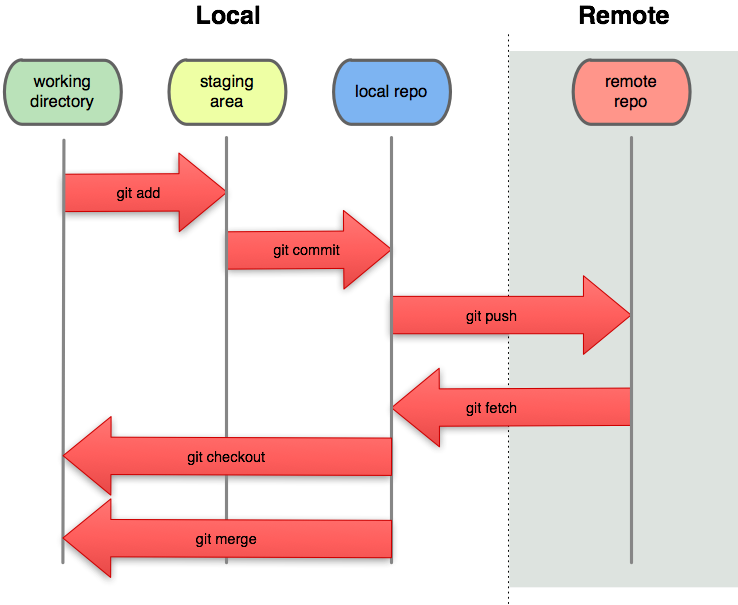
\includegraphics[width=0.45\textwidth]{images/local-remote}
      \caption{Local and Remote operations in Git. \cite{whygitisbetterthanx}}
      \label{local-remote}
    \end{figure}

    \begin{itemize}
      \item Fast access to old revisions.  Since the repository is hosted
      locally it is only hard drive access time slowing it down instead of
      network access times.
      \item Always accessible.  Even if you don't have internet or the central
      server is down you can always commit to your own repository.
    \end{itemize}

    Generally in an organizational context a central server will still be used
    with the DVCS system.  This way everyone has a single source so they can
    keep their code tightly integrated and reduce the headaches introduced of
    their repositories diverge too much.

    Comparing the workflow mentioned above on a DVCS it would go as follows:
    The developer updates their clone of the repository to the latest version.
    They then do the changes to implement whatever feature they are working on.
    These changes are committed to their local repository, this always succeeds
    since they are the only ones with access to it.  They then push this
    changeset up to the central server.  If no-one else has pushed this succeeds
    and the central server will be at the same version as their repository.  If
    someone else has pushed to the central server then they will have to pull
    the changeset and merge it into their repository.  One of the key
    differences at this point is that their change has been committed and can
    trivially be recovered if something goes wrong.  Once they resolve the merge
    they create a new merge commit that has both their change and the other
    change that was pushed to the server as parents.  They can then push this
    change up to the central server (assuming no one else has pushed during this
    time).
